\chapter{Experiments}
\label{ch:experiments}

In this chapter an experiment is presented in order to assert the quality of the proposed planning system. The experiment presents the advantage of the blending of pushing and grasping actions. 

The experiment (Figure \ref{fig:experiment_good}) presents all the challenges the planners can handle, which are: objects on top of others and objects that need to be moved in order to grasp them. 
\begin{figure}[tb]
\centering
\begin{subfigure}[t]{0.45\textwidth}
\centering
\includegraphics[height=5cm]{Img/experiments/image.png}
\caption{Kinect's view}\label{fig:experiment_good1}
\end{subfigure}
\begin{subfigure}[t]{0.45\textwidth}
\centering
\includegraphics[height=5cm]{Img/experiments/image_labels.png}
\caption{Objects labels.}\label{fig:experiment_good2}
\end{subfigure}
\caption{Kinect's view of the first experiment.}\label{fig:experiment_good}
\end{figure}


\iffalse
%reference: http://tex.stackexchange.com/questions/53061/insert-image-and-list-inside-a-table
\begin{table}[!h]
\begin{center}
\begin{tabular}{>{\centering\arraybackslash}m{3cm} >{\centering\arraybackslash}m{3cm} >{\centering\arraybackslash}m{3cm} >{\centering\arraybackslash}m{3cm} }
%{>{\centering}m{1in} >{\centering}m{lin} >{\centering}m{lin} >{\centering}m{lin}}
\toprule 
Iteration & Action & Action execution & Result\\
\cmidrule(r){1-1}\cmidrule(lr){2-2}\cmidrule(lr){3-3}\cmidrule(l){4-4}
1 &
\ttt{(push\_dir3 o2)} 
& 
\includegraphics[height=23mm]{Img/experiments/exp_good/action1c.png}
&
\includegraphics[height=23mm]{Img/experiments/result1.png}
\\
2 &
\ttt{(grasp o2)} 
& 
\includegraphics[height=23mm]{Img/experiments/exp_good/action2c.png}
&
\includegraphics[height=23mm]{Img/experiments/result2.png}
\\
3 &
\ttt{(push\_dir1 o1)} 
& 
%\raisebox{-\totalheight}{
\includegraphics[height=23mm]{Img/experiments/exp_good/action3c.png}%}
&
\includegraphics[height=23mm]{Img/experiments/result3.png}
\\
4 &
\ttt{(push\_dir1 o0)} 
& 
\includegraphics[height=23mm]{Img/experiments/exp_good/action4c.png}
&
\includegraphics[height=23mm]{Img/experiments/result4.png}
\\
5 &
\ttt{(grasp o4)} 
& 
\includegraphics[height=23mm]{Img/experiments/exp_good/action5c.png}
&
\includegraphics[height=23mm]{Img/experiments/result5.png}
\\
6 &
\ttt{(grasp o1)} 
& 
\includegraphics[height=23mm]{Img/experiments/exp_good/action6c.png}
&
\includegraphics[height=23mm]{Img/experiments/result6.png}
\\
7 &
\ttt{(grasp o3)}
& 
\includegraphics[height=23mm]{Img/experiments/exp_good/action7c.png}
&
\includegraphics[height=23mm]{Img/experiments/result7.png}
\\
8 &
\ttt{(grasp o0)} 
& 
\includegraphics[height=23mm]{Img/experiments/exp_good/action8c.png}
&
\includegraphics[height=23mm]{Img/experiments/result8.png}
\\
9 &
\ttt{(grasp o5)} 
& 
\includegraphics[height=23mm]{Img/experiments/exp_good/action9c.png}
&
\includegraphics[height=23mm]{Img/experiments/result9.png}
\end{tabular}
\end{center}
\caption{Sequence of action for the experiment of Figure \ref{fig:experiment_good2}}\label{tab:experiment_good}
\end{table}
\fi

\begin{figure}
\centering
\begin{subfigure}[t]{\textwidth}
\begin{subfigure}[t]{0.195\textwidth}
\centering 
\includegraphics[width=\textwidth]{Img/experiments/exp_good/action1c.png}
\end{subfigure}
\begin{subfigure}[t]{0.195\textwidth}
\centering 
\includegraphics[width=\textwidth]{Img/experiments/exp_good/action2c.png}
\end{subfigure}
\begin{subfigure}[t]{0.195\textwidth}
\centering 
\includegraphics[width=\textwidth]{Img/experiments/exp_good/action3c.png}
\end{subfigure}
\begin{subfigure}[t]{0.195\textwidth}
\centering 
\includegraphics[width=\textwidth]{Img/experiments/exp_good/action4c.png}
\end{subfigure}
\begin{subfigure}[t]{0.195\textwidth}
\centering 
\includegraphics[width=\textwidth]{Img/experiments/exp_good/action5c.png}
\end{subfigure}
\\
\begin{subfigure}[t]{0.195\textwidth}
\centering 
\stackunder[5pt]	{\includegraphics[width=\textwidth]{Img/experiments/result1.png}}{\ttt{(push\_dir3 o2)}}
\end{subfigure}
\begin{subfigure}[t]{0.195\textwidth}
\centering 
\stackunder[5pt]	{\includegraphics[width=\textwidth]{Img/experiments/result2.png}}{\ttt{(grasp o2)} }
\end{subfigure}
\begin{subfigure}[t]{0.195\textwidth}
\centering 
\stackunder[5pt]	{\includegraphics[width=\textwidth]{Img/experiments/result3.png}}{\ttt{(push\_dir1 o1)} }
\end{subfigure}
\begin{subfigure}[t]{0.195\textwidth}
\centering 
\stackunder[5pt]	{\includegraphics[width=\textwidth]{Img/experiments/result4.png}}{\ttt{(push\_dir1 o0)} }
\end{subfigure}
\begin{subfigure}[t]{0.195\textwidth}
\centering 
\stackunder[5pt]	{\includegraphics[width=\textwidth]{Img/experiments/result5.png}}{\ttt{(grasp o4)} }
\end{subfigure}
\end{subfigure}
\vspace{1cm}
\begin{center}
\begin{subfigure}[t]{\textwidth}
\centering
\begin{subfigure}[t]{0.195\textwidth}
\centering 
\includegraphics[width=\textwidth]{Img/experiments/exp_good/action6c.png}
\end{subfigure}
\begin{subfigure}[t]{0.195\textwidth}
\centering 
\includegraphics[width=\textwidth]{Img/experiments/exp_good/action7c.png}
\end{subfigure}
\begin{subfigure}[t]{0.195\textwidth}
\centering 
\includegraphics[width=\textwidth]{Img/experiments/exp_good/action8c.png}
\end{subfigure}
\begin{subfigure}[t]{0.195\textwidth}
\centering 
\includegraphics[width=\textwidth]{Img/experiments/exp_good/action9c.png}
\end{subfigure}
\\
\begin{subfigure}[t]{0.195\textwidth}
\centering 
\stackunder[5pt]	{\includegraphics[width=\textwidth]{Img/experiments/result6.png}}{\ttt{(grasp o1)} }
\end{subfigure}
\begin{subfigure}[t]{0.195\textwidth}
\centering 
\stackunder[5pt]	{\includegraphics[width=\textwidth]{Img/experiments/result7.png}}{\ttt{(grasp o3)}}
\end{subfigure}
\begin{subfigure}[t]{0.195\textwidth}
\centering 
\stackunder[5pt]	{\includegraphics[width=\textwidth]{Img/experiments/result8.png}}{\ttt{(grasp o0)}}
\end{subfigure}
\begin{subfigure}[t]{0.195\textwidth}
\centering 
\stackunder[5pt]	{\includegraphics[width=\textwidth]{Img/experiments/result9.png}}{\ttt{(grasp o5)}}
\end{subfigure}
\end{subfigure}
\end{center}

\caption{Results of a run for the experiment of Figure \ref{fig:experiment_good}. The executed plan is: \ttt{(push\_dir3 o2)} 
\ttt{(grasp o2)} 
\ttt{(push\_dir1 o1)} 
\ttt{(push\_dir1 o0)} 
\ttt{(grasp o4)} 
\ttt{(grasp o1)} 
\ttt{(grasp o3)}
\ttt{(grasp o0)} 
\ttt{(grasp o5)}. The first and third row of images show the robot executing the actions, while below the results of those actions.}\label{fig:execution_experiment}
\end{figure}

In Figure \ref{fig:execution_experiment} the execution of the plan and the results of each action are shown. The plan first decides to push away object \ttt{o2} since it is not able to grasp it due to its grasping pose. In that pose the Kinect is able to see also a side of the object, and therefore its second and third principal components make the grasping pose being the one in Figure \ref{fig:exp_good_grasp_o2}, which is colliding which object \ttt{o3}. Therefore it has to move object \ttt{o3}, but it cannot because \ttt{o2} hinders that action, another option is pushing away \ttt{o2} and then grasp it. In the next iteration the system takes a new image and the grasping pose of \ttt{o2} has no collisions, and the system decides to grasp it. Then it pushes away object \ttt{o1} because it is not possible to grasp it or to move the other objects having \ttt{o1} in such a position. Next it pushes object \ttt{o0}, this action shows the optimality of the planner. If it did not push \ttt{o0} it had to push away first \ttt{o5} and \ttt{o3} to make \ttt{o0} graspable, it saved one action pushing away \ttt{o0}. The outcome of this action is not the expected one since the gripper, during the pushing action, touched slightly also \ttt{o5} (Figure \ref{fig:pushing_o0}). In this case is possible noting the ability of the system to adapt to unexpected outcomes. Then the robot finishes the task grasping the remaining objects.



\begin{figure}
\centering
\begin{subfigure}[t]{0.45\textwidth}
\centering
\includegraphics[width = 5.5cm]{Img/experiments/exp_good/grasp_o2.png}
\caption{}
\end{subfigure}
\begin{subfigure}[t]{0.45\textwidth}
\centering
\includegraphics[width = 5.5cm]{Img/experiments/exp_good/grasp_o2_2.png}
\caption{}
\end{subfigure}
\caption{Collision between the gripper and \ttt{o3} for the grasping pose of object \ttt{o2}.}\label{fig:exp_good_grasp_o2}
\end{figure}

\begin{figure}[tb]
\centering
\includegraphics[width=6cm]{Img/experiments/exp_good/pushing_o0c.png}
\caption{Unexpected outcome: pushing \ttt{o0} the gripper touches also \ttt{o5}.}\label{fig:pushing_o0}
\end{figure}

In order to get some statistics regarding the planning system we performed 6 runs of the experiment. All the times commented refer about an execution on a machine with dual-core CPU with $3.16GHz$. In Table \ref{tab:6runs} the executed plans of all the runs are reported. The plans are different because of two main reasons: the segmentation is not always the same and in the attempt to reproduce the experiment the objects could have been not positioned in the same poses of previous experiments. 

From these experiments it has been noted that the segmentation have a strongly importance since, due to the noise of the Kinect, the segmentation was not always the same, despite the filtering. Also the tuning of the segmentation parameters made it quite noisy sensitive. Moreover, at the edges the segmentation algorithm had some drawbacks since it could cluster some edges points to the biggest adjacent clusters of supervoxels, this means that some edges of an object could be detected as part of the adjacent object. This, in several situation, can leads to find no plan since the object model is not similar to the real object, and during the computation of the collisions the system could detect false collisions. In this case the system can either return no solution, so it will take a new images and repeat all the process (the new segmentation could solve the problem), or find anyway a plan.  




%%%%%%%%%%% MY COMMENT: The total time here takes into account that the wrong segmentation cases were neglected and also the time needed to save the point clouds
\begin{table}
\caption{Executed plans of the 6 runs for the experiment of Figure \ref{fig:experiment_good}. $N_{actions}$ is the total number of executed actions, $Time_{tot}$ is the total time to solve the task (neglecting the time lost due to the bad segmentation), $\neg Solution$ is the number of iterations in which no solution was found because of the segmentation and $\neg IK$ is the number of actions that had no solution for the inverse kinematic and the system replaned.}\label{tab:6runs}
\begin{center}
\begin{tabular}{>{\centering\arraybackslash}m{1.5cm} >{\centering\arraybackslash}m{8cm} >{\centering\arraybackslash}m{1.5cm} >{\centering\arraybackslash}m{1.5cm} >{\centering\arraybackslash}m{1.5cm} >{\centering\arraybackslash}m{1cm}}
\toprule 
Run & Plan & $N_{actions}$ & $Time_{tot}$ & $\neg Solution$ & $\neg IK$\\
%\cmidrule(r){1-1}\cmidrule(lr){2-2}\cmidrule(l){3-3}
\toprule
1 & 
\ttt{(push\_dir3 o2)} 
\ttt{(push\_dir1 o1)} 
\ttt{(grasp o1)} 
\ttt{(push\_dir1 o5)} 
\ttt{(grasp o5)} 
\ttt{(push\_dir3 o2)} 
\ttt{(push\_dir1 o0)} 
\ttt{(grasp o0)} 
\ttt{(grasp o3)}
\ttt{(grasp o2)} 
\ttt{(grasp o4)} 
& 11 & $404.9s$ & 3 & 6\\
\toprule
2 &
\ttt{(push\_dir3 o2)} 
\ttt{(grasp o2)} 
\ttt{(push\_dir2 o1)} 
\ttt{(grasp o1)} 
\ttt{(grasp o4)} 
\ttt{(push\_dir2 o0)} 
\ttt{(grasp o0)} 
\ttt{(grasp o3)} 
\ttt{(grasp o5)} 
& 9 & $263.2s$ & 19 & 0\\
\toprule
3 & 
\ttt{(push\_dir3 o2)} 
\ttt{(grasp o2)} 
\ttt{(grasp o4)} 
\ttt{(push\_dir2 o1)} 
\ttt{(grasp o1)} 
\ttt{(push\_dir1 o0)} 
\ttt{(grasp o0)} 
\ttt{(grasp o3)} 
\ttt{(grasp o5)} 
& 9 & $306.2s$ & 3 & 1\\
\toprule
4 & 
\ttt{(grasp o2)} 
\ttt{(grasp o4)} 
\ttt{(push\_dir1 o3)} 
\ttt{(grasp o3)} 
\ttt{(push\_dir1 o1)} 
\ttt{(grasp o1)} 
\ttt{(push\_dir1 o5)} 
\ttt{(grasp o5)} 
\ttt{(grasp o0)} 
& 9 & $266.7s$ & 0 & 0
\\
\toprule
5 &
\ttt{(push\_dir3 o2)} 
\ttt{(grasp o4)} 
\ttt{(push\_dir1 o1)} 
\ttt{(grasp o1)} 
\ttt{(push\_dir1 o5)} 
\ttt{(grasp o5)} 
\ttt{(push\_dir1 o0)} 
\ttt{(grasp o0)} 
\ttt{(grasp o3)} 
\ttt{(grasp o2)} 
& 10 & $283.9s$ & 0 & 0\\
\toprule
6 & 
\ttt{(push\_dir3 o2)} 
\ttt{(grasp o2)} 
\ttt{(push\_dir1 o1)} 
\ttt{(push\_dir1 o0)} 
\ttt{(grasp o4)} 
\ttt{(grasp o1)} 
\ttt{(grasp o3)}
\ttt{(grasp o0)} 
\ttt{(grasp o5)} 
& 9 & $262.1s$ & 6 & 0\\
\toprule
\end{tabular}
\end{center}
\end{table}

\paragraph{Comments}
In run 1 the robot grasps object \ttt{o3} although there was \ttt{o4} on top of it. This is because during the execution of \ttt{(push\_dir1 o0)}  action the gripper's cable touched object \ttt{o4} moving it away.  In runs 1, 4 and 5 the optimal plan does not return to push object \ttt{o0} as a solution but it returns to push either \ttt{o5} or \ttt{o3}, this also is because of the segmentation (at that iteration that system detected that it was not possible pushing away \ttt{o0}). 


\begin{figure}[tb]
\centering
\begin{subfigure}[t]{0.45\textwidth}
\centering
\includegraphics[width=6cm]{Img/experiments/exp_good/grasp_o4.png}
\end{subfigure}
\begin{subfigure}[t]{0.45\textwidth}
\centering
\includegraphics[width=6cm]{Img/experiments/exp_good/grasp_o4_rviz.png}
\end{subfigure}
\caption{Grasping pose of object \ttt{o4} with unfeasible IK.}\label{fig:grasp_o4}
\end{figure}

Due to the strange position of object \ttt{o4} the grasping poses some times were the one depicted in Figure \ref{fig:grasp_o4}. When the planner returned to grasp \ttt{o4} the inverse kinematic returned no solution, so it planed again performing a different action. The unfeasible grasping pose for object \ttt{o4} was due to the height of the object which was higher than its width, so the second principal direction was perpendicular to the top largest surface (Figure \ref{fig:grasp_o4}). The situation was solved by taking new images, the Kinect was not able to see well the side of object \ttt{o4} so sometimes the computed grasping pose could have solution. This can be easily solved by using more sophisticated grasping planning algorithms. 
\todo[inline]{This thing about the grasping pose of \ttt{o4} is worthy to mention?}

\begin{figure}[tb]
\centering
\begin{subfigure}[t]{0.4\textwidth}
\centering
\includegraphics[height=6.5cm]{Img/experiments/exp_good/data/filtering.eps}
\caption{Filtering time in seconds.}
\end{subfigure}
\begin{subfigure}[t]{0.4\textwidth}
\centering
\includegraphics[height=6.5cm]{Img/experiments/exp_good/data/segmentation.eps}
\caption{Segmentation time in milliseconds.}
\end{subfigure}
\\
\begin{subfigure}[t]{0.45\textwidth}
\centering
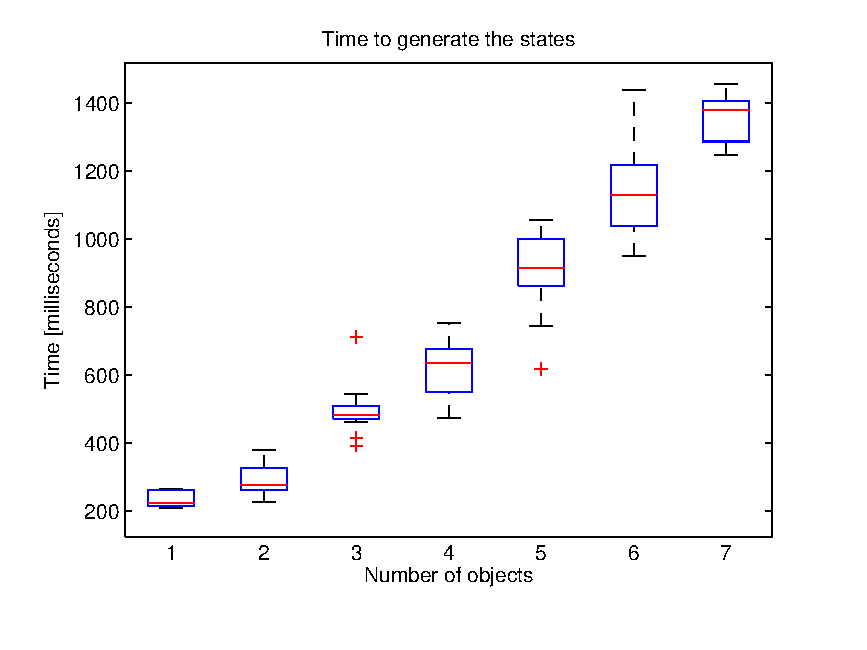
\includegraphics[width=\textwidth]{Img/experiments/exp_good/data/predicates.eps}
\caption{State generation time in milliseconds.}
\label{fig:time_predicates}
\end{subfigure}
\begin{subfigure}[t]{0.45\textwidth}
\centering
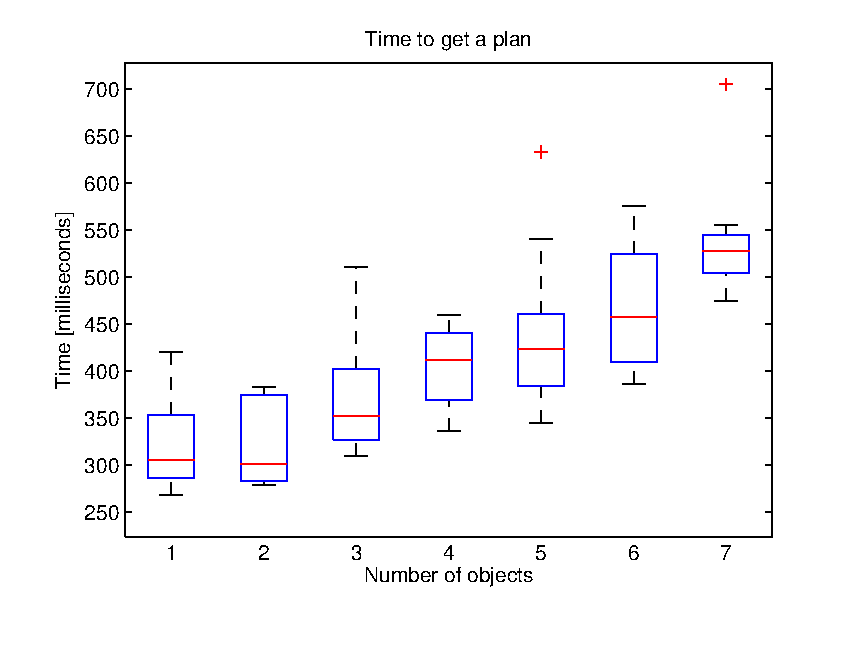
\includegraphics[width=\textwidth]{Img/experiments/exp_good/data/planning.eps}
\caption{Planning time in milliseconds.}\label{fig:time_plan}
\end{subfigure}
\\
\begin{subfigure}[t]{0.45\textwidth}
\centering
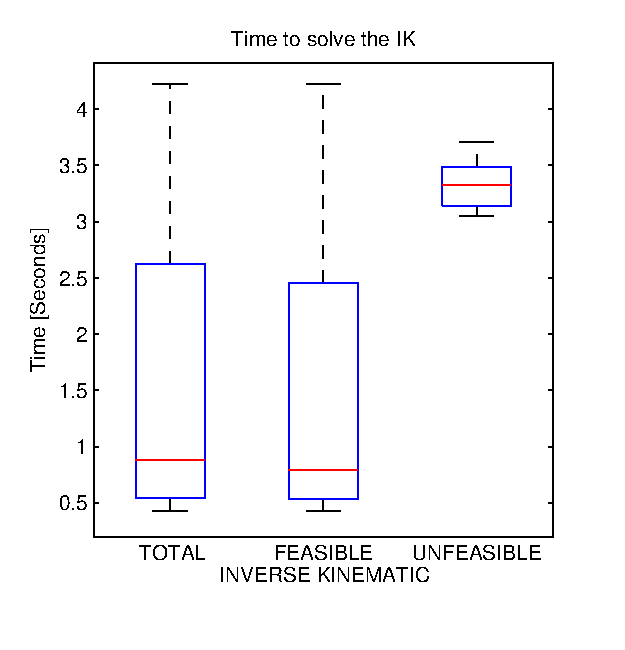
\includegraphics[height=6.5cm]{Img/experiments/exp_good/data/ik.eps}
\caption{Inverse kinematic time in seconds.}
\end{subfigure}
\begin{subfigure}[t]{0.45\textwidth}
\centering
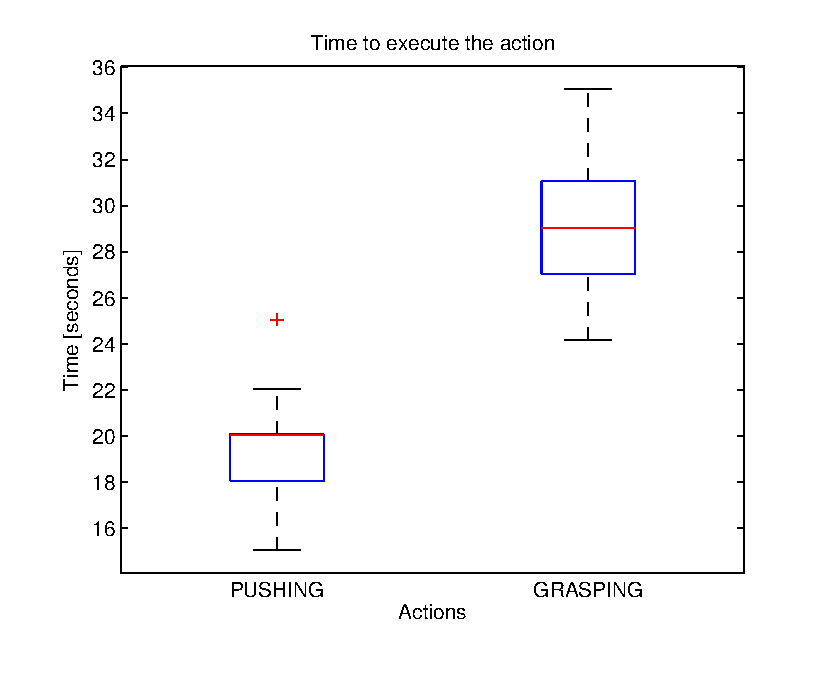
\includegraphics[height=6.5cm]{Img/experiments/exp_good/data/actions.eps}
\caption{Action execution time in seconds.}
\end{subfigure}
\caption{Elapsed time for the different phases of the algorithm. These data are taken from the 6 runs of the experiment of Figure \ref{fig:experiment_good}.}\label{fig:time_results}
\end{figure}
% COMMENT ABOUT THE FIGURE: I took data also from runs where the segmentation was wrong and no plan was found. For example in those cases it is anyway usefull to use the data of the elapsed times for the segmentation/state generation/planning, but not for executed actions since no actions was performed, or for the IK since without a plan we don't solve IK. In this way we are able to have a more precise estimation of the elapsed time since we have more data. Despite this, for example for the case of the state generation time, each box was not obtained with the same number of data. 


\paragraph{Computation time analysis}
From the 6 runs of this experiment the different elapsed times for the several steps of the algorithm have been measured (Figure \ref{fig:time_results}). The planning system is slowed down by the filtering process ($\approx 2.2sec$), therefore other filtering algorithms should be considered. The segmentation is really fast since in average it takes half second to segment the image.

The most important part of this analysis regards the time needed to generate the states and get a plan (Figures \ref{fig:time_predicates} and \ref{fig:time_plan}). The planning system is able to compute the predicates quite fast and, as commented in Chapter \ref{ch:implementation}, its complexity is $\mathcal{O}(n^2)$. The time to get a plan depends on the complexity of the problem, that is on the number of objects. The Fast Downward planner showed to be very fast in resolving also complex problems with 7 objects. It is important also taking into account that our implementation to get the plan is not the optimal one since we write each time a PDDL file and then call the binary file of the planner. Hence, the process is slowed down by the writing of the PDDL file and the parsing of that file, and a better implementation should be considered. Despite this, the time to get a plan is few.

Regarding the time needed to compute the inverse kinematic is considerable and there is a big variance due to the fact that there exist poses for which is easier to find a solution and others for which is harder. 

The execution of the actions is obviously the more expensive. The grasping actions takes more time than pushing since it is composed of more steps.

In Figure \ref{fig:pipeline} the execution times per iteration of the perception and planning pipeline are depicted. We can observe that the whole system takes about $\approx 4.5 seconds$ to take a decision after receiving a point cloud. The contribution of this thesis is at the level of planning and at the high level of the perception (i.e. the generation of the states), therefore the attention should be focused on the box regarding the state generation and the planning pipeline. Neglecting the filtering and the segmentation the system takes $\approx 2.3 seconds$ to make a decision. Moreover, the IK depends on the robot and on the implementation, therefore we also showed the time performance neglecting the time to compute the inverse kinematic. It is possible observing that the system is fast since it takes in average 1 second, from the segmentation of the objects, to decide what action to do. 

To conclude, we present in Figure \ref{fig:run6_time} the elapsed times for the different phases of the proposed planning system for the $6$-th run of the experiment. From that graph is appreciable that the worst part of the planning system is due to the low level perception (filtering and segmentation). The state generation takes some time for complex problems but for simple problems it is very efficient. 


\begin{figure}
\centering
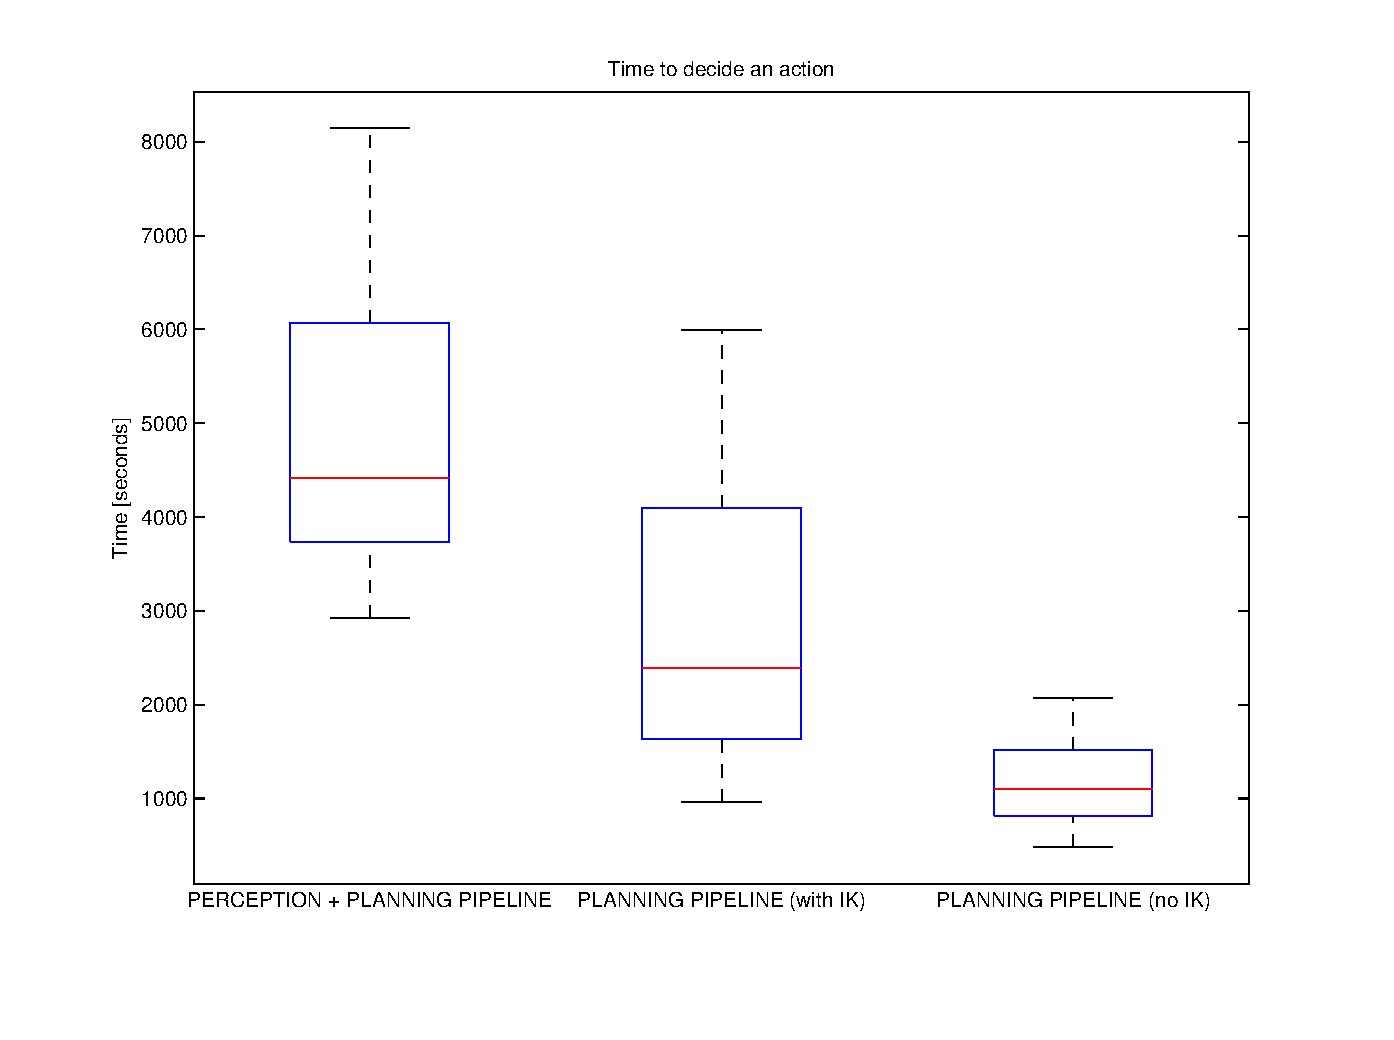
\includegraphics[width=16cm]{Img/experiments/exp_good/data/pipeline.eps}
\caption{Time in seconds of the execution of the perception and planning pipelines. Those execution times are retrieved by all the runs without taking care about the number of segmented objects.}\label{fig:pipeline}
\end{figure}

\begin{figure}
\centering
\begin{subfigure}[t]{0.48\textwidth}
\centering
\includegraphics[width=9.1cm]{Img/experiments/exp_good/data/exp_times_with_actions.eps}
\caption{}\label{fig:run6_time_actions}
\end{subfigure}
\begin{subfigure}[t]{0.48\textwidth}
\centering
\includegraphics[width=9.5cm]{Img/experiments/exp_good/data/exp_times_no_actions.eps}
\caption{}  \label{fig:run6_time_no_actions}
\end{subfigure}
\caption{Execution time for the different steps of the pipeline for the $6$-th run of the experiment. Figure \ref{fig:run6_time_actions} includes the execution of the actions, while Figure \ref{fig:run6_time_no_actions} does not include the execution of the actions. }\label{fig:run6_time}
\end{figure}


\iffalse
In this chapter the performance of the proposed task planner for the considered task is evaluated by performing several experiments with the aim to study the quality, its benefits and its limitations.

To get the quality of the task planner the strategy defined in the article \citep{Benchmarking} by Amignoni et al. In that article they proposed a general method to evaluated the quality of a task planner. 
First they define a functionality benchmark\footnote{A functionality benchmark is a benchmark of specific robotic task. In the case of this thesis a benchmark of the task planner.} thought 4 elements:
\begin{itemize}
\item Description: a high level, general, description of the functionality
\item Input/Output: the information available to the module implementing the function-
ality when executed, and the expected outcome.
\item Benchmarking data: the data needed to perform the evaluation of the performance
of the functional module.
\item Metrics: algorithms to process benchmarking data in an objective way.
\end{itemize}

Regarding the benchmarking of a task planner those elements are defined as:
\begin{itemize}
\item [\textbf{Description:}] Given a initial state and a goal state find a set of actions to reach the goal.
\item [\textbf{Input/Output:}] The inputs are the PDDL domain and problem descriptions. The output is a plan expressed as sequence of actions.
\item [\textbf{Benchmarking data:}] Some data has to be supplied by the robot, including: the input
given to the planner, the output (i.e., the plan) delivered by the planner, and the
performance data for the planner (e.g., memory and time needed). According to
the planning approach, other data might be required. Other data will be possibly collected when a plan is
actually executed, including: time needed to execute each action and time needed
to execute the whole plan.
\item [\textbf{Metrics:}] Metrics are mainly related to good plan quality and to solving time. The target of benchmarking task planning is twofold: to asses the quality of the
plan produced (e.g., in terms of the cost for executing it and its likelihood to succeed) and to assess the quality of the
planning process (i.e., how fast is the plan generated and how much resources are needed to do so). Possible metrics are:
\begin{itemize}
\item \textsl{Levenshtein distance}\footnote{\href{https://en.wikipedia.org/wiki/Levenshtein_distance} {https://en.wikipedia.org/wiki/Levenshtein\_distance}} is a metric that specifies the distance between two strings, in this case a plan can be though as a sequence of character, where each action with a determined object of interest is a character of the string. The Levenshtein distance between the two lists is calculated to measure the quality of the plan. Levenshtein distance
$L_{A,B}(|A|,|B|)$ between two lists A and B is calculated as
\begin{align*}
L_{A,B}(i,j) &= \max(i,j) \qquad if \quad \min(i,j)=0 \\
L_{A,B}(i,j) &= \min(L_{A,B}(i-1,j)+1, \\
& \qquad \quad L_{A,B}(i,j-1)+1,
\\ & \qquad \quad L_{A,B}(i-1,j-1)+1_{a_i \neq b_i})
\qquad otherwise
\end{align*}
where $|A|$ is the length of plan A, and $1_{a_i \neq b_i}$ is equal to 0 if the action $a_i$ is the same of action $b_i$. This metric will be used to evaluate the distance between the optimal plan returned by the planner in the first frame and the real executed plan. 
\item Number of actions correctly performed in the correct order (e.g., number of
objects delivered to their correct destination). 
\item Time required to construct a plan and time to perform it. 
\end{itemize}
\end{itemize}
We will also evaluate the difference of executing the initial plan and executing the plan with the replanning technique in terms of time and number of correct actions. As well also the number of bad, or dangerous, object manipulations due to the lack of replanning, lack of probability and geometric constraints in the planner . 

It is important highlighting that what has been done is not a benchmarking since no comparison is done with other state of the art planners, but the commented guideline for benchmarks has been used in order to get some useful metrics in order to assert the quality of the planner. 

Kinds of possible experiment to do:
\begin{itemize}
\item show experiments first trying only separating the object (infinite loop behaviour) and then coupling the grasping action. 
\item Show the results of the planner with the pushing length chosen not accordingly to the surrounding objects but accordingly to the pushed one. From that comment the improvements.
\item Show normal experiment where everything works
\item Show situation why we are going to consider the risk as cost in the action. 
\end{itemize}

Metrics to considers:
\begin{itemize}
\item number of objects
\item segmentation time
\item Total solution time
\item planning time
\item total solution
\item Inverse kinematics solution time (this will probably used to justify the backtracking method)
\item Predicates time computation (maybe add collision checking time in )
\end{itemize}


Find a way to get the computational complexity. 

\begin{figure}
\centering
\includegraphics[width=\textwidth]{Img/general/experiments.png}
\end{figure}

\begin{itemize}
\item 2 experiments in which everything works
\item experiment which shows the limitaiton of the planner
\end{itemize}

\fi